\section{From local seed hits to candidate mappings}
\label{sec:chaining-purpose}

When minimizers are generated and we take the intersection (by hash value) of the minimizer sets between the query and the reference, we get a set of seed hits which is encoded as anchors.

\section{Anchor geometry and ordering}
\label{sec:chaining-geometry}

A seed hit is represented by an anchor
\[
  a_i=(r_i,q_i,\sigma_i,\ell_i,g_i,\phi_i),
\]
where \(r_i\) and \(q_i\) are inclusive seed-end coordinates on the reference
and query, \(\sigma_i\) is the strand, \(\ell_i\) is the query span, \(g_i\)
identifies a query segment, and \(\phi_i\) stores additional ordering flags.

Below you can see the physical representation of the anchor in memory in minimap2 and in our implementation. We could potentially use adaptive representation similar to minimizers, but anchors are fewer than minimizers, so the benefit would be limited for additional complexity of C++ templates.

\begin{BioseqCppSnippet}
  typedef struct {
    uint32_t n;                    (*@\BioseqCodeNote{Size of cr array (number of matches in the reference sequence)}@*)
    uint32_t q_pos;                (*@\BioseqCodeNote{Query position}@*)
    uint32_t q_span       : 31;    (*@\BioseqCodeNote{Query minimizer span in symbols}@*)
    uint32_t flt          : 1;     (*@\BioseqCodeNote{If the minimizer is filtered out (very frequently occuring in the reference sequence)}@*)
    uint32_t seg_id       : 31;    (*@\BioseqCodeNote{Query segment identifier}@*)
    uint32_t is_tandem    : 1;     (*@\BioseqCodeNote{Tandem repeat flag}@*)
    const uint64_t *cr;            (*@\BioseqCodeNote{Multiple reference coordinates per anchor}@*)
  } mm_seed_t;
\end{BioseqCppSnippet}
\begin{BioseqCppSnippet}
  struct anchor {
    std::uint64_t ref_position;    (*@\BioseqCodeNote{Absolute reference coordinate}@*)
    std::uint64_t query_position;  (*@\BioseqCodeNote{Absolute query coordinate}@*)
    std::uint32_t is_reverse;      (*@\BioseqCodeNote{Reverse-strand flag encoded as zero or one}@*)
    std::uint8_t query_span;       (*@\BioseqCodeNote{Query minimizer span in symbols}@*)
    std::uint8_t flags;            (*@\BioseqCodeNote{Seed flags propagated by collection}@*)
    std::uint16_t segment_id;      (*@\BioseqCodeNote{Query segment identifier}@*)
  };
\end{BioseqCppSnippet}

\todo{Improve anchor API}

Figure~\ref{fig:chaining-dotplot} shows viasual interpretation. Valid
anchors that can be used for chaining lie below and to the left of the current anchor. A chain can move
between nearby diagonals to represent an insertion or deletion, but large
diagonal changes receive a penalty or are not considered at all.

\begin{figure}[tbp]
\centering
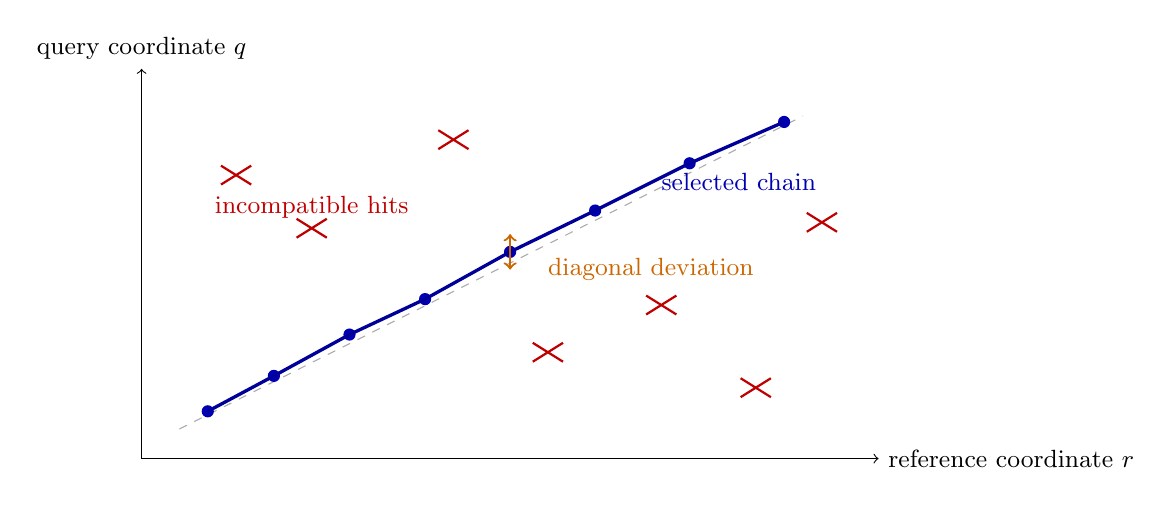
\begin{tikzpicture}[x=0.12cm,y=0.075cm,font=\small]
  \draw[->] (0,0) -- (78,0) node[right] {reference coordinate \(r\)};
  \draw[->] (0,0) -- (0,66) node[above] {query coordinate \(q\)};
  \draw[dashed,gray!65] (4,5) -- (70,58);
  \foreach \x/\y in {7/8,14/14,22/21,30/27,39/35,48/42,58/50,68/57}
    \fill[blue!70!black] (\x,\y) circle (2.2pt);
  \draw[very thick,blue!60!black]
    (7,8)--(14,14)--(22,21)--(30,27)--(39,35)--(48,42)--(58,50)--(68,57);
  \foreach \x/\y in {10/48,18/39,33/54,43/18,55/26,65/12,72/40}
    \draw[red!75!black,thick] (\x-1.6,\y-1.6)--(\x+1.6,\y+1.6)
      (\x-1.6,\y+1.6)--(\x+1.6,\y-1.6);
  \draw[<->,orange!80!black,thick] (39,32) -- (39,38);
  \node[orange!80!black,anchor=west] at (42,32)
    {diagonal deviation};
  \node[blue!70!black,below right] at (54,50) {selected chain};
  \node[red!75!black,above] at (18,39) {incompatible hits};
\end{tikzpicture}
\caption{Chaining selects growing, approximately
collinear path so we can get closer to the final result. Base-level alignment (later stage of the pipeline) will later resolve gaps between anchors.}
\label{fig:chaining-dotplot}
\end{figure}

\info{Why we look for anchors that are colinear?}{In the perfect scenario without gaps \(r_i-q_i\) is constant. An increasing diagonal coordinate indicates that in reference we matched more symbols than in the query (meaning insertion/deletion has occured). Chaining needs to specify costs for abandoning the main diagonal too much (intuitevely we don't want the case in which we introduce very large gap in the reference sequence just to match one or two symbols in the query, because it's improbable that some very large fragment was replaced during evolutionary processes by just a few bases)}

As we would like to have some well defined order of anchors, we sort them by strand and reference coordinate first, then by the additional metadata:
\begin{equation}
\begin{split}
 K_r(a_i) &=
   (\sigma_i \ll 63)\mathbin{\vert}
   \bigl(r_i\mathbin{\&}(2^{63}-1)\bigr),\\
 K_q(a_i) &=
   (g_i\ll48)\mathbin{\vert}(\phi_i\ll40)
   \mathbin{\vert}(\ell_i\ll32)
   \mathbin{\vert}(q_i\bmod 2^{32}).
\end{split}
\label{eq:chaining-order}
\end{equation}

Comparison is lexicographic in \(K_r\), \(K_q\), and the full \(q_i\). The hashing doesn't need full 64 bits for query position i.e if query coordinates $q_i$ exceed \(2^{32}\) we still have correct order as the leftmostpart is still the fragment number $g_i$ (fragments won't be larger than $2^{32}$). Fragmentation of sequences is discussed later in the storage chapter.

The ordering is required, because the chaining wants to process anchors in sequential order (increasing query positions), while we build chains of anchors using reference positions.

\section{Intuitive interpretation}
\label{sec:chaining-interpretation}

We need to first understand how intuitively human would align sequences. First we choose a random fragment of query and use text search in our editor to find that exact fragment. The longer fragment is better, because it's less likely that we found it just because of random subsitutions ocurring.
At first we won't find it, but we repeatadly delete chacters from the fragment start or end until match is found. Each match corresponds to possible location in the target sequence.
If we repat the process enough for other fragments of query we will establih the most probable locations of query in the target sequence (by seeing groups of matches). Throughout this chapter we will never gave any reason to treat query
and target asymetrically as  scoring functions don't distinguish between both inputs. The distinction was rather coming from their role in the alignment flow
(the larger set of sequences can be called the set of references or targets, while the smaller one could be called queries).

\info{Longest increasing sequence}{If the reference coordinates are increasing, then naive approach would be finding LIS (longest increasing subsequence) of query coordinates. You can think of the chaining as "improving" this simplistic approach by changing query coordinates to more complex scoring function which can handle gaps and other complex cases.}

The sorting mentioned in section~\ref{sec:chaining-geometry} is required, because what we would like to intuitively do is check where the first reference fragment can be placed in query sequence and when we move to the next anchor (increasing reference positon), the position of query should increase too (logically if the middle of query matches somewhere, then we should see the end of it, not the beggining).
This introduces some emergent assymetry: it will be very likely to see one anchor in query matched with multiple anchors in referece (query can occur multiple times in reference), however what happens if one reference fragment is matched to multiple query fragments?
This situation means that is hard to distinguish which part of the query is best to match:
\begin{itemize}
  \item $\text{Reference}\gets XYZVW, \text{Query}\gets YZV$ - it's immediately obvious that for $V$ in the reference we found the end of query
  \item $\text{Reference}\gets XYZVW, \text{Query}\gets VXVXVXV$ - we don't know what part (is this start or the end of query, or the middle part?) we should consider without looking at neighbours of $V$.
\end{itemize}

\warn{Emergent assymetry}{In the following chapters I will present new optimisations that are not discussed in the field of computational biology. The emergent assymetry will play important role when talking about the experimental results in separate chapter~\ref{sec:chaining-cpu-experimental-analysis}.} 

\section{Chaining components}

We defined the anchors that are input to chaining pipeline stage, however chaining itself isn't a monolith. It can be viewed as composition of several steps. 

\info{Chaining pipeline}{Although chaining can be decomposed into several steps that are dispatched to differrent functions, in BioseqDB this is an internal implementation detail and we don't allow users to alter for example which backtracking backend is used (although we could expose parts of chaining as composable components in the future)}

Forward chaining (which is the core component) produces the score array \(f\) and predecessor array \(p\). Second most important step is backtracking (as typically in case of DP algorithms which fill some state matrices) reads the sorted anchors, \(f\), and \(p\). The backtracking writes theflat output
anchor array supplied by the caller, denoted by \(A\) ($A$ can be viewed as type \texttt{anchor A\[\]}).

The chaining can be fully decomposed into the following steps:
\begin{enumerate}
  \item \textbf{Forward chaining} reads the sorted anchors and writes the
    temporary \(f\) and \(p\) arrays.
  \item \textbf{Backtracking} reads these inputs and writes the accepted chain
    records plus full anchor copies in \(A\).
  \item \textbf{Region generation} converts each chain record into one
    alignment region while retaining \(A\).
  \item \textbf{Region selection} filters the regions while
    retaining \(A\).
  \item \textbf{Base-level alignment} reads the selected regions, their slices
    of \(A\), the query and target sequences, and the alignment parameters. It
    fills the base-level fields in the regions supplying exact start/end coordinates, match qualities etc.
\label{list:chaining-components}
\end{enumerate}

BioseqDB represents every chain record with the following structure:
\begin{BioseqCppSnippet}
  struct chain {
    int32_t score        = 0;    (*@\BioseqCodeNote{Accepted-chain score}@*)
    int32_t anchor_count = 0;    (*@\BioseqCodeNote{Anchors in the chain}@*)
    int32_t anchor_start = 0;    (*@\BioseqCodeNote{Start of the chain slice in A}@*)
  };
\end{BioseqCppSnippet}
Where \texttt{anchor\_start} is the index of the first anchor in the chain in the array \(A\).

For a non-empty
record \(c\), its anchors occupy consecutive positions in forward order:
\[
  A[c.\texttt{anchor\_start}],\ldots,
  A[c.\texttt{anchor\_start}+c.\texttt{anchor\_count}-1].
\]

The array \(A\) is constructed using $f$ and $p$ arrays. For every anchor \(i\), the two stored values mean:
\begin{description}
  \item[\(f_i\)] the score of the best chain that the selected forward
    algorithm found with anchor \(i\) at its end.
  \item[\(p_i\)] the index of the anchor immediately before \(i\) in that
    chain. The value is \(-1\) when the best chain found for \(i\) starts at
    \(i\)
\end{description}
For example,
\[
  p_7=5,\qquad p_5=2,\qquad p_2=-1
  \quad\Longrightarrow\quad
  7\to5\to2\to-1.
\]

\raggedbottom

\definecolor{chainGray}{HTML}{A0A0A0}
\definecolor{chainBlue}{HTML}{4C78A8}
\definecolor{chainOrange}{HTML}{F28E2B}
\definecolor{chainGreen}{HTML}{59A14F}
\tikzset{
  chain stage/.style={draw=black!65,fill=gray!7,rounded corners,
    align=center,minimum height=.78cm,inner sep=4pt},
  chain blue/.style={chain stage,draw=chainBlue!90!black,fill=chainBlue!11},
  chain orange/.style={chain stage,draw=chainOrange!90!black,fill=chainOrange!14},
  chain green/.style={chain stage,draw=chainGreen!80!black,fill=chainGreen!12},
  chain muted/.style={chain stage,draw=chainGray!85!black,fill=chainGray!12},
  chain flow/.style={-{Latex[length=1.8mm]},thick},
  chain soft flow/.style={-{Latex[length=1.6mm]},thick,draw=chainGray!90!black},
  chain point/.style={circle,draw=chainBlue!90!black,fill=chainBlue!18,
    minimum size=.38cm,inner sep=0pt},
  chain current/.style={circle,draw=chainOrange!95!black,very thick,
    fill=chainOrange!20,minimum size=.48cm,inner sep=0pt}
}

\section{Chaining algorithms}
\label{sec:chaining-algorithm-families}

Similar to the minimizer chapter here we will discuss different approaches to chaining. The algorithm itself is based on dynamic programming scoring, but the details differ.

\begin{table}[H]
\centering
\caption{Comparison of different chaining algorithms}
\label{tab:chaining-algorithm-taxonomy}
\footnotesize
\setlength{\tabcolsep}{3.2pt}
\renewcommand{\arraystretch}{1.10}
\begin{tabularx}{\linewidth}{@{}
  >{\raggedright\arraybackslash}p{0.07\linewidth}
  >{\raggedright\arraybackslash}p{0.23\linewidth}
  >{\raggedright\arraybackslash}X
  >{\raggedright\arraybackslash}p{0.26\linewidth}@{}}
\toprule
\textbf{ID} & \textbf{Algorithm} & \textbf{Defining decision} &
\textbf{Implementations}\\
\midrule
B1 & Ordered predecessor scan & Visit recent candidates first. Increase the
skip counter when a marked candidate does not improve the score. Decrease a
positive counter after an improvement. Stop when the counter exceeds its
limit. Also score cached predecessor \(m\) when it exists and the main scan
does not reach it
& minimap2 non-RMQ chaining, BioSeqDB scalar and exact SIMD\\
B2 & Source-to-target DP & Apply each completed source score in parallel
to later targets admitted by the kernel's index and distance checks
& G3SA first CUDA pass\\
B3 & Ranking-value second pass & Rank predecessors by a value calculated from
their saved scores and coordinates. Keep at most one predecessor with the
largest accepted ranking value. If one was saved, calculate its full pair
score & G3SA second CUDA pass\\
B4 & Range-minimum-query tree DP & Use a balanced tree whose nodes cache the
smallest stored priority in each subtree, then calculate the full score for the
selected predecessor & minimap2 RMQ and BioSeqDB's experimental RMQ route,
which includes both query-coordinate boundaries and omits the bandwidth check\\
B5 & Per-element batch-limited DP & Keep one running score for each vector
element. Stop after enough consecutive batches leave all of those scores unchanged &
BioSeqDB bounded CPU SIMD\\
B6 & Per-target batch-limited DP & Keep one best score for the target.
Stop after enough consecutive batches fail to increase that score & BioSeqDB Vulkan\\
\bottomrule
\end{tabularx}
\end{table}

Scalar and exact SIMD both implement B1 because they make the same ordered
decisions. G3SA selects a short kernel or one of two tiled launch
configurations according to range size within B2 and B3. BioSeqDB CPU SIMD and
Vulkan use different batch stopping rules, so they are B5 and B6.

All implementations pass their saved scores and predecessors to later code
that builds and classifies mappings.

The BioSeqDB RMQ implementation includes both query-coordinate boundaries. It can
select a predecessor with the same query coordinate as the target and accept
it without a bandwidth test. We classify the tree design as B4 and describe
these defects in
Section~\ref{sec:chaining-bioseqdb}.

\subsection{Shared pair score}

Let's say we have two anchors with coordinates $q_j, q_i$ and $r_j, r_i$ on the query and reference.
Let's assume the minimizer span is always $k$. We now can say that after incorporating $(r_j, r_i)$ anchor we will cover $q_i-q_j$ symbols on the query and $r_i-r_j$ symbols on the reference, however those two jumps can be interpreted as
taking some symbols from query and assuming they form replacement and the rest forms a gap. For example let's say $q_i-q_j > r_i-r_j$. This means that we match more symbols in query than in reference, so indicates some deletion in the reference.
So we can say $r_i-r_j$ symbols are replaced (or stay the same) while the leftover $(q_i-q_j)-(r_i-r_j)$ symbols form this deletion. This thinking is symmetrical so we just only need to use minimum and absolute value to make it more generic.

Now we introduced $g(j,i)$ (the advance shared by the reference and query) and $\delta(j,i)$ (the remaining advance in whichever sequence moves farther).
As k-mers represent hashed fragment of length $k$ we can assume that in our match we have exactly $\min\{q_i-q_j, r_i-r_j, k\}$ new symbols that matched.
Hence we now define our first primitive score as $\min\{q_i-q_j, r_i-r_j, k\} = \min\{g(j,i), k\}$.

This scoring has some problems with the most important one being that it doesn't penalize the case when we have a large gap in the reference sequence just to match one or two symbols in the query. This is improbable that some very large fragment was replaced during evolutionary processes by just a few bases.
For that reason we will use function $\left\lfloor\text{Penalty}(\delta, g)\right\rfloor$. The penalty function should satisfy the following properties:
\begin{itemize}
  \item There's no penalty for doing nothing at all: $\text{Penalty}(0, 0) = 0$
  \item For $g \leq k \land \delta = 0$ there's no gap so there's shouldn't be any penalty: $\text{Penalty}(0, g) = 0$
  \item Penalty should be monotonically increasing with respect to $\delta$: $\text{Penalty}(\delta, g) \leq \text{Penalty}(\delta+1, g)$
  \item Penalty should be increasing slower than linearly with respect to $g$: $\text{Penalty}(\delta, g+1) < \text{Penalty}(\delta, g) + 1$. This guarantees that increasing $g$ without touching $\delta$ benefits overall score (we prefer replacement region over gap region)
  \item For small $g$ and $\delta$ our penalty function should prefer increase in $g$ rather than $\delta$. This is equivalent of saying that we want to stay close to the diagonal and reduce the gap size introduced: $\text{Penalty}(\delta+1, g) \geq \text{Penalty}(\delta, g+1)$
  \item For large $g$ and $\delta$ our penalty function should be asymptotically the same for both $\delta$ and $g$. This is equivalent of saying that if we encounter very large gaps, then it doesn't matter if we increase the matching region between two fragments or increase the gap as both fragments are very dissimilar: $O_{\delta}(\text{Penalty}(\delta, g = \text{const})) = O_{g}(\text{Penalty}(\delta = \text{const}, g))$
\end{itemize}

\info{Symmetry}{Using $g$ and $\delta$ as only parameters for penalty function guarantees that scoring is symmetric. Symmetry makes sure that gap costs are the same for both query and reference.}

Our final score is then something of the following structure:
\begin{equation}
\begin{gathered}
\text{Score}(j,i) = \min\{g(j,i), k\} - \left\lfloor\text{Penalty}(\delta(j,i), g(j,i))\right\rfloor \\
= \min\{g(j,i), k\} - \left\lfloor \alpha * g(j,i) + \beta * \delta(j,i) + \gamma * f(\delta(j,i)) \right\rfloor \\
0 \leq \alpha, \beta, \gamma \leq 1
\end{gathered}
\end{equation}

\begin{figure}[tbp]
\centering
\begin{tikzpicture}[x=.34cm,y=.34cm,font=\footnotesize,>=Latex,
  dist axis/.style={-{Latex[length=1.4mm]},thin},
  dist common/.style={-{Latex[length=1.7mm]},very thick,
    draw=chainGreen!80!black},
  dist excess/.style={-{Latex[length=1.7mm]},very thick,
    draw=chainOrange!95!black},
  dist measure/.style={<->,thin,draw=chainBlue!90!black},
  dist summary/.style={draw=black!55,fill=gray!4,rounded corners=0pt,
    text width=3.75cm,align=center,inner sep=3pt}]

  \begin{scope}[xshift=0cm]
    \node[font=\bfseries,align=center,text width=4.5cm] at (4.3,12.0)
      {(a) Both advances\\are below \(k\)};
    \draw[dist axis] (-.15,0)--(9.4,0) node[below right] {\(r\)};
    \draw[dist axis] (0,-.15)--(0,9.5) node[above left] {\(q\)};
    \node[chain point,label=below left:\(a_j\)] (d1j) at (0,0) {};
    \node[chain current,label=above right:\(a_i\)] (d1i) at (3,3) {};
    \draw[dist common] (d1j)--node[midway,above left] {\(g=3\)} (d1i);
    \node[text=chainOrange!95!black,anchor=west] at (3.8,3.0)
      {\(\delta=0\)};
    \draw[dist measure] (0,-1.05)--node[midway,below] {\(d_r=3\)}
      (3,-1.05);
    \draw[dist measure] (-1.05,0)--node[midway,left] {\(d_q=3\)}
      (-1.05,3);
    \node[dist summary] at (4.25,-4.6)
      {\(g=3,\ \delta=0\)\\reward \(\min(g,k)=3\)};
  \end{scope}

  \begin{scope}[xshift=5.0cm]
    \node[font=\bfseries,align=center,text width=4.5cm] at (4.3,12.0)
      {(b) Reference moves\\much farther};
    \draw[dist axis] (-.15,0)--(9.4,0) node[below right] {\(r\)};
    \draw[dist axis] (0,-.15)--(0,9.5) node[above left] {\(q\)};
    \node[chain point,label=below left:\(a_j\)] (d2j) at (0,0) {};
    \coordinate (d2g) at (2,2);
    \node[chain current,label=above right:\(a_i\)] (d2i) at (8,2) {};
    \draw[dist common] (d2j)--node[midway,above left] {\(g=2\)} (d2g);
    \draw[dist excess] (d2g)--node[midway,above] {\(\delta=6\)} (d2i);
    \draw[dist measure] (0,-1.05)--node[midway,below] {\(d_r=8\)}
      (8,-1.05);
    \draw[dist measure] (-1.05,0)--node[midway,left] {\(d_q=2\)}
      (-1.05,2);
    \node[dist summary] at (4.25,-4.6)
      {\(g=2,\ \delta=6\)\\reward \(\min(g,k)=2\)};
  \end{scope}

  \begin{scope}[xshift=10.0cm]
    \node[font=\bfseries,align=center,text width=4.5cm] at (4.3,12.0)
      {(c) Both advances\\exceed \(k\)};
    \draw[dist axis] (-.15,0)--(9.4,0) node[below right] {\(r\)};
    \draw[dist axis] (0,-.15)--(0,9.5) node[above left] {\(q\)};
    \node[chain point,label=below left:\(a_j\)] (d3j) at (0,0) {};
    \coordinate (d3g) at (7,7);
    \node[chain current,label=above right:\(a_i\)] (d3i) at (8,7) {};
    \draw[dist common] (d3j)--node[midway,above left] {\(g=7\)} (d3g);
    \draw[dist excess] (d3g)--node[midway,below] {\(\delta=1\)} (d3i);
    \draw[dist measure] (0,-1.05)--node[midway,below] {\(d_r=8\)}
      (8,-1.05);
    \draw[dist measure] (-1.05,0)--node[midway,left] {\(d_q=7\)}
      (-1.05,7);
    \node[dist summary] at (4.25,-4.6)
      {\(g=7,\ \delta=1\)\\reward \(\min(g,k)=5\)};
  \end{scope}
\end{tikzpicture}
\caption{Three anchor displacements for \(k=5\). The blue brackets are the
actual reference and query advances. The green diagonal step advances both
coordinates by \(g=\min(d_r,d_q)\). The orange horizontal step is the
remaining \(\delta=|d_r-d_q|\). It would be vertical when \(d_q>d_r\).
Panel (c) also shows that the reward stops at \(k\), even though \(g>k\).}
\label{fig:chaining-distance-examples}
\end{figure}

The minimap2 scoring definition $E$ looks exactly as what we have just specified:
\begin{equation}
\begin{aligned}
 d_q(j,i) &= q_i-q_j, & d_r(j,i) &= r_i-r_j,\\
 \delta(j,i) &= \lvert d_r(j,i)-d_q(j,i)\rvert,
 & g(j,i) &= \min\{d_r(j,i),d_q(j,i)\}.
\end{aligned}
\label{eq:chaining-distances}
\end{equation}

\begin{equation}
 E(j,i)=\min\{\ell_j,g(j,i)\}-P(j,i),
\label{eq:chaining-link-score}
\end{equation}
where
\begin{equation}
P(j,i)=
\begin{cases}
0,
  & \delta(j,i)=0\ \land\ g(j,i)\leq\ell_j,\\[2pt]
\left\lfloor
  \lambda_g\delta(j,i)+\lambda_s g(j,i)
  +\dfrac{1}{2}\operatorname{mglog}_{2}\!\bigl(\delta(j,i)+1\bigr)
\right\rfloor,
  & \text{otherwise}.
\end{cases}
\label{eq:chaining-penalty}
\end{equation}
The function \(\operatorname{mglog}_{2}\) is minimap2's polynomial
approximation of \(\log_2\). So far in the abstract definition of scoring we didn't mention diagonal, but nonnegative coefficient \(\lambda_g\) can be viewed as diagonal-gap penalty (further away from diagonal we penalize more), where the nonnegative coefficient \(\lambda_s\) is the penalty for distance. The value \(\ell_j\) is the
query span of predecessor \(j\). (In our example above we used $k$ for all k-mers sizes, but as mentioned before minimap2 with specific settings can compress regions of same repeating symbols so we just replace $k$ with kmer span $\ell_j$. All the logic stays the same) \coderef{minimap2/lchain.c}
{Minimap2 chaining link score}{comput_sc}{113}

\info{Score units}{In this definition we view scoring function as expressed in number of matched symbols (not some arbitrary large numbers), so the coefficients must be set accordingly so the values are scaled correctly. In the dynamic programming formulation we then can take maximum of $E$ value and $\ell_i$ to make sure that in the worst case scenario we assume that we at least matched the length of the minimizer. There are no formal limitations on this normalization, but it makes reasoning about the scores easier.}

It's worth noting that defined scoring is also symmetrical in terms of coordinates i.e the score doesn't take $r_i, q_i$ positions as parameters so reversing coordinate systems doesn't change the outcome.
However, in dynamic programming we often want to use the locally close predecessor as the best one. 

We see that scoring is not easy to work with as it depends on both anchors. If we used a linear gap scoring similar to what we discussed in alignment foundations chapter~\ref{sec:alignment-model} we would get a score that is not dependent on both anchors.
Note that the following is true due to trivial relationship between arithmetic average, distance and minimum:
\begin{equation}
\begin{aligned}
  \phi(j, i) = \frac{d_q(j,i) + d_r(j,i)}{2} \\
  \delta(j,i) + 2*g(j,i) = \phi(j,i)
\end{aligned}
\end{equation}
So we can simplify our scoring function to be only dependent on $\phi(j,i)$ (I replaced $min(\ell_j, g(j,i))$ with just $\ell_j$ and replaced penalty function with a simple linear function dependent on $\phi(j,i)$):
\begin{equation}
\begin{aligned}
  E(j,i) = \ell_j - \lambda_{\phi} * \phi(j,i)
\end{aligned}
\end{equation}
Now if we assume that every anchor has constant span (as most of them will have length $k$), then we can define:
\begin{equation}
\begin{aligned}
  f_j = \max_{i < j}\{f_i+E(j,i)\}, \\
  \text{GlobalScore}(i) &= f_i + \lambda_{\phi} * (q_i + r_i)
\end{aligned}
\label{eq:global-score-definition-chaining-rmq}
\end{equation}
We can observe that:
\begin{equation}
\begin{aligned}
  f_i+E(j,i) > f_k+E(k,i) \iff \\
  f_i + \ell_j - \lambda_{\phi} * \phi(j,i) > f_k + \ell_k - \lambda_{\phi} * \phi(k,i) \iff \\
  \text{GlobalScore}(i) + \ell_j > \text{GlobalScore}(k) + \ell_k \iff \\
  \text{GlobalScore}(i) > \text{GlobalScore}(k)
\end{aligned}
\end{equation}
This means that we can compute $\text{GlobalScore}(i)$ independently for each anchor and use it to calculate global score.
This is what was done in minimap2 as described in minigraph paper~\cite{minimap2_rmq_scoring_minigraph}.
The problem is that the new linear gap scoring is very simplistic and does not exhibit some of the properties I discussed earlier.

\begin{figure}[tbp]
\centering
\begin{tikzpicture}[x=.38cm,y=.38cm,font=\footnotesize,>=Latex,
  link axis/.style={-{Latex[length=1.4mm]},thin},
  link path/.style={-{Latex[length=1.8mm]},very thick,
    draw=chainGreen!80!black},
  link measure/.style={<->,thin,draw=chainBlue!90!black},
  link summary/.style={draw=black!55,fill=gray!4,rounded corners=0pt,
    text width=5.0cm,align=center,inner sep=3pt}]

  \begin{scope}[xshift=0cm]
    \node[font=\bfseries] at (5.0,11.0) {(a) Close predecessor};
    \draw[link axis] (-.15,0)--(11.0,0) node[below right] {reference \(r\)};
    \draw[link axis] (0,-.15)--(0,10.2) node[above left] {query \(q\)};
    \draw[dashed,draw=chainGray!80!black] (1,0)--(11,10);
    \node[chain point,label={left:\(a_{j_{\mathrm{near}}}=(7,6)\)}]
      (nearj) at (7,6) {};
    \node[chain current,label={above right:\(a_i=(10,9)\)}]
      (neari) at (10,9) {};
    \draw[link path] (nearj)--node[midway,above left] {\(g=3\)}
      (neari);
    \draw[link measure] (7,-1.0)--node[midway,below] {\(d_r=3\)}
      (10,-1.0);
    \draw[link measure] (10.75,6)--node[midway,right] {\(d_q=3\)}
      (10.75,9);
    \node[link summary] at (5.0,-4.5)
      {same diagonal: \(\delta=0\)\\link advances 3 positions in each sequence};
  \end{scope}

  \begin{scope}[xshift=7.6cm]
    \node[font=\bfseries] at (5.0,11.0) {(b) Far predecessor};
    \draw[link axis] (-.15,0)--(11.0,0) node[below right] {reference \(r\)};
    \draw[link axis] (0,-.15)--(0,10.2) node[above left] {query \(q\)};
    \draw[dashed,draw=chainGray!80!black] (1,0)--(11,10);
    \node[chain point,label={above left:\(a_{j_{\mathrm{far}}}=(2,1)\)}]
      (farj) at (2,1) {};
    \node[chain current,label={above right:\(a_i=(10,9)\)}]
      (fari) at (10,9) {};
    \draw[link path] (farj)--node[midway,above left] {\(g=8\)}
      (fari);
    \draw[link measure] (2,-1.0)--node[midway,below] {\(d_r=8\)}
      (10,-1.0);
    \draw[link measure] (10.75,1)--node[midway,right] {\(d_q=8\)}
      (10.75,9);
    \node[link summary] at (5.0,-4.5)
      {same diagonal: \(\delta=0\)\\link advances 8 positions in each sequence};
  \end{scope}
\end{tikzpicture}
\caption{A close and a far predecessor for the same current anchor
\(a_i=(10,9)\). Both candidates lie on the diagonal \(r-q=1\), so both have
\(\delta=0\). Their link lengths are nevertheless different: the close link
has \(g=3\), whereas the far link has \(g=8\). Thus zero diagonal deviation
does not mean zero or equal distance.}
\label{fig:chaining-near-far-distance}
\end{figure}

